\documentclass[11pt]{article}
\usepackage{fontspec}
\usepackage{xcolor}
\definecolor{darkblue}{rgb}{0,0,0.5}
\usepackage[colorlinks=true,allcolors=darkblue]{hyperref}
\usepackage{amsmath}
\usepackage{amssymb}
\usepackage{booktabs}
\usepackage{multirow}
\usepackage{enumitem}
\setlist{noitemsep}
\usepackage[font=small]{caption}
\usepackage{graphicx}
\usepackage[sorting=ynt,style=authoryear,uniquename=false]{biblatex}
\addbibresource{bachelor_thesis.bib}
\usepackage{tikz-dependency}
\date{August 2017}
\title{Encoding morphological annotations for universal dependency parsing}
\begin{document}
\maketitle
\begin{center}
  \vfill
  \textit{Author:}\\\smallskip
  \textbf{Kuan Yu}\\\smallskip
  \texttt{kuan.yu@student.uni-tuebingen.de}\\\vfill
  \textit{Advisor:}\\\smallskip
  \textbf{Dr.~Çağrı Çöltekin}\\\smallskip
  \texttt{ccoltekin@sfs.uni-tuebingen.de}\\\vfill
\end{center}

\begin{abstract}
  We investigated different methods of encoding morphological annotations for the neural network classifier in a transition-based dependency parser.
  The most effective and efficient method we found was embedding morphological entries as real vectors
  which compose through a simple componentwise operation such as max.
\end{abstract}

\section{Introduction}
\label{sec:intro}

Morphological annotations provide valuable linguistic information.
Figure~\ref{fig:feats} gives an example for the word ``am'',
annotated by an attribute-value structure (AVS) with five entries,
where each entry is an attribute-value pair.

\begin{figure}[htb!]
  \centering
  \texttt{Mood=Ind|Number=Sing|Person=1|Tense=Pres|VerbForm=Fin}
  \caption[]{\label{fig:feats}Morphological AVS for ``am''.}
\end{figure}

Encoding such structured information in machine learning for language processing is however not entirely straightforward.
The number of entries in a morphological AVS is uncertain.
In English, it ranges from zero (such as for prepositions) to five and more.
It is also difficult to determine when a morphological attribute is applicable,
simply based on the word form or the word class.
Consider for the verb ``like'',
the \texttt{Person} attribute is applicable in ``I like'' and ``He likes'' but not in ``He does like''.

We investigated different methods of encoding morphological annotations for machine learning,
and evaluated these methods in the task of universal dependency parsing.
Our program is open source under the MIT license.%
\footnote{\url{https://github.com/ysmiraak/darc}}

We will first describe the parsing task (Section~\ref{sec:ud}--\ref{sec:nnc}),
then our methods (Section~\ref{sec:embed}--\ref{sec:feats}),
and finally our experiments and the results (Section~\ref{sec:res}--\ref{sec:conc}).

\section{Universal dependencies}
\label{sec:ud}

Universal Dependencies (UD) \parencite{ud} is a cross-linguistically consistent annotation scheme for dependency-based treebanks.%
\footnote{\url{http://universaldependencies.org}}
UD treebanks conform to the CoNLL-U format.%
\footnote{\url{http://universaldependencies.org/format.html}}
In this format, each node in a dependency-graph has ten fields named
\texttt{ID}, \texttt{FORM}, \texttt{LEMMA}, \texttt{UPOSTAG}, \texttt{XPOSTAG}, \texttt{FEATS}, \texttt{HEAD}, \texttt{DEPREL}, \texttt{DEPS}, and \texttt{MISC}.
A labeled directed arc \(label(parent, child)\) is given by \(DEPREL(HEAD, ID)\).
Figure~\ref{fig:tree} gives an example of a dependency tree.
The arc \(conj(1,6)\) crosses \(root(0,2)\) as well as \(punct(2,9)\),
making this tree non-projective.

\begin{figure}[htb!]
  \centering
  \begin{dependency}[theme=simple, label style={font=\ttfamily\normalsize}]
    \begin{deptext}[font=\ttfamily\footnotesize, column sep=1.5em]
      Darc \&stays \&the \&parse \&and \&full \&of \&errors \&.\\
    \end{deptext}
    \depedge{2}{1}{xcomp}
    \deproot[edge unit distance=4ex]{2}{root}
    \depedge{4}{3}{det}
    \depedge{2}{4}{nsubj}
    \depedge{6}{5}{cc}
    \depedge[segmented edge, label style={below}, edge unit distance=2.4ex, edge start x offset=-0.7em]{1}{6}{conj}
    \depedge{8}{7}{case}
    \depedge{6}{8}{obl}
    \depedge[segmented edge, label style={below}, edge unit distance=1.2ex]{2}{9}{punct}
  \end{dependency}
  \caption[]{\label{fig:tree}A non-projective dependency tree.\\\\
    \centering\ttfamily\tiny
    \begin{tabular}{lllllll}
      ID &FORM &LEMMA &UPOSTAG &FEATS &HEAD &DEPREL\\
      \midrule
      1 &Darc   &darc  &ADJ     &Degree=Pos                                            &2 &xcomp\\
      2 &stays  &stay  &VERB    &Mood=Ind|Number=Sing|Person=3|Tense=Pres|VerbForm=Fin &0 &root\\
      3 &the    &the   &DET     &Definite=Def|PronType=Art                             &4 &det\\
      4 &parse  &parse &NOUN    &Number=Sing                                           &2 &nsubj\\
      5 &and    &and   &CCONJ   &\_                                                    &6 &cc\\
      6 &full   &full  &ADJ     &Degree=Pos                                            &1 &conj\\
      7 &of     &of    &ADP     &\_                                                    &8 &case\\
      8 &errors &error &NOUN    &Number=Plur                                           &6 &obl\\
      9 &.      &.     &PUNCT   &\_                                                    &2 &punct\\
    \end{tabular}}
\end{figure}

From UD version 2.0 (UD2) \parencite{ud20data, ud20testdata},
we selected 15 treebanks representing a variety of language families and morphological typologies,
although fusional Indo-European languages are the most available choices.
Our selections also vary in sizes and degrees of non-projectivity.
Each treebank consists of a train-, a dev-, and a test-set.
Table~\ref{tab:ds} lists the statistics from the train-sets.

\begin{table}[htb!]
  \centering
  {\ttfamily\small
    \begin{tabular}{lccccc}
      \toprule
      treebank &\#tree &\#node &\%nonp &family &type\\
      \midrule
      Ancient\_Greek &11\,476 &159\,895 &62.77 &IE.Hellenic     &fus\\
      Arabic         &~6\,075 &223\,881 &10.77 &AA.Semitic      &fus\\
      Basque         &~5\,396 &~72\,974 &33.52 &Vasconic        &agg\\
      Bulgarian      &~8\,907 &124\,336 &~3.17 &IE.Balto-Slavic &fus\\
      Chinese        &~3\,997 &~98\,608 &~0.63 &Sino-Tibetan    &iso\\
      Croatian       &~7\,689 &169\,283 &~8.56 &IE.Balto-Slavic &fus\\
      Dutch          &12\,330 &186\,467 &20.28 &IE.Germanic     &fus\\
      Finnish-FTB    &14\,981 &127\,602 &~7.47 &Uralic          &agg\\
      Hebrew         &~5\,241 &137\,680 &~1.26 &AA.Semitic      &fus\\
      Italian        &12\,838 &270\,703 &~4.24 &IE.Italic       &fus\\
      Latin-PROIEL   &14\,192 &147\,044 &26.52 &IE.Italic       &fus\\
      Persian        &~4\,798 &121\,064 &~6.86 &IE.Iranian      &fus\\
      Polish         &~6\,100 &~62\,501 &~0.85 &IE.Balto-Slavic &fus\\
      Swedish        &~4\,303 &~66\,645 &~3.18 &IE.Germanic     &fus\\
      Turkish        &~3\,685 &~38\,082 &11.23 &Turkic          &agg\\
      \bottomrule
    \end{tabular}}
  \caption[]{\label{tab:ds}
    \footnotesize
    \begin{tabular}{rl}
      \texttt{\#tree} &number of trees\\
      \texttt{\#node} &number of syntactic nodes\\
      \texttt{\%nonp} &percentage of non-projective trees\\
      \texttt{family} &\texttt{IE}: Indo-European, \texttt{AA}: Afro-Asiatic\\
      \texttt{type}   &\texttt{iso}: isolating, \texttt{agg}: agglutinative, \texttt{fus}: fusional\\
    \end{tabular}}
\end{table}

\section{Transition-based parsing}
\label{sec:pars}

Dependency parsing produces a directed acyclic graph from a sequence of nodes \([w_{0}, w_{1}, \ldots, w_{n}]\),
which are the syntactic tokens of a sentence,
where \(w_{0}\) is a pseudo root node.
A transition-based parsing algorithm defines transition actions over configurations.
Each configuration is a triple consisting of a stack \(\sigma\), a buffer \(\beta\), and a set of arcs \(A\).
From the initial configuration \((\sigma \colon [w_{0}], \beta \colon [w_{1}, w_{2}, \ldots, w_{n}], A \colon \{\})\),
a series of transition actions are taken to produce a terminal configuration \((\sigma \colon [w_{0}], \beta \colon [\,], A)\).

We adopted a non-projective variant of the arc-standard algorithm \parencite{nivre2008algorithms, nivre2009non}.
The transition actions are listed below.
For labeled parsing, some actions are parameterized over \(arc\), the set of possible dependency labels,
in which case a different action is defined for each label.

\begin{align*}
  \mathtt{shift} &:& (\sigma, [w_{i} \vert \beta], A) &\mapsto ([w_{i} \vert \sigma], \beta, A)& &\\
  \mathtt{left(arc)} &:& ([w_{i}, w_{j} \vert \sigma], \beta, A) &\mapsto ([w_{i} \vert \sigma], \beta, A \cup \{arc(w_{i}, w_{j})\})& &\\
  \mathtt{right(arc)} &:& ([w_{i}, w_{j} \vert \sigma], \beta, A) &\mapsto ([w_{j} \vert \sigma], \beta, A \cup \{arc(w_{j}, w_{i})\})& &0 \neq j\\
  \mathtt{swap} &:& ([w_{i}, w_{j} \vert \sigma], \beta, A) &\mapsto ([w_{i} \vert \sigma], [w_{j} \vert \beta], A)& &0 < j < i\\
\end{align*}

A classifier is trained for estimating the probabilities of each transition action given the current state of the configuration.
For training the classifier, we implemented the static oracle designed by \textcite{nivre2009improved}.
The static oracle produces a transition sequence which leads to the gold-standard parse of a sentence.
Details about the classifier is discussed in Section~\ref{sec:nnc}.
Our parser is greedy, which means that only the most probable legal transition action is taken.

The parsing results are evaluated the same way as in the CoNLL 2017 Shared Task: Multilingual Parsing from Raw Text to Universal Dependencies \parencite{udst:overview}.
The evaluation metric is the labeled attachment score (LAS),
namely the percentage of syntactic nodes with the correct HEAD and DEPREL\@.
Non-syntactic nodes in the CoNLL-U format, i.e.\ empty nodes and multi-word tokens, are simply ignored.
Only the UD labels count for scoring, and not the language-specific subtypes.
For example, \texttt{acl:relcl} is considered to be the same as \texttt{acl}.
However, our parser always keeps the complete DEPREL given by the treebank.

In UD, a sentence has a single root,
which means that a unique syntactic node is attached to the pseudo root node.
However, the transition algorithm may attach multiple ones.
Our parser keeps the first attachment, and re-attach the other nodes to the first one with a \texttt{parataxis} arc.

\section{Neural network classifier}
\label{sec:nnc}

Following \textcite{chen2014fast}, we implemented a simple feedforward neural network classifier
in Keras \parencite{chollet2015keras} with the TensorFlow backend \parencite{tensorflow2015-whitepaper}.

The input features are extracted from 18 graph nodes.

\begin{itemize}
\item 3 nodes from the stack top, with the top two being the nodes of interest
\item 3 lookaheads from the buffer
\item 2 leftmost \& rightmost children of the two
\item 1 leftmost-of-leftmost \& rightmost-of-rightmost children of the two
\end{itemize}

Some nodes may be missing in a configuration,
in which case dummy values are supplied as input features.

The inputs are successively transformed by two hidden layers each with 256 rectified linear units (ReLU),
and then outputted through a softmax layer with as many units as transition actions.
The softmax output assigns a probability for each action.
Successive layers are fully connected.
The weights for the connections are initialized in a random uniform distribution following \textcite{he2015delving}.
The parameters are updated through backpropagation using the AdaMax algorithm \parencite{kingma2014adam} in batches of 32 training instances,
with 25\% dropout \parencite{srivastava2014dropout} applied to the hidden layers.%
\footnote{We experimented with a higher dropout rate,
  and found that while it could improve the accuracy of the model slightly,
  it also required extending the sizes of the layers,
  which would quadratically increase the number of parameters.}

\section{Nominal features}
\label{sec:embed}

All the input features for our classifier are nominal values, i.e.\ symbols.

\begin{itemize}
\item Lexical features: FORM \& LEMMA
\item Part-of-speech information: UPOSTAG
\item Morphological information: FEATS
\item Partial graph information: DEPREL, from the children nodes
\end{itemize}

Table~\ref{tab:ds:stats} lists some statistics about these nominal categories.
Details about FEATS are discussed in Section~\ref{sec:feats}.
Analogously to word classes,
UPOSTAG and DEPREL are closed in the sense that new members are not expected,
while FORM and LEMMA are open classes for assuming Zipfian distributions where the majority of the members appear only once or twice.
Since an open nominal class anticipates new symbols which are unseen in the training data,
we add a catch-all symbol for unknowns,
and all symbols with unique appearances are replaced with it for parameter training.

\begin{table}[htb!]
  \centering
  {\small\ttfamily
    \begin{tabular}{lcccccc}
      \toprule
      treebank &\#upos &\#drel &\#form &\#form* &\#lemma &\#lemma*\\
      \midrule
      Ancient\_Greek &14 &25 &33\,237 &11\,856 &10\,932 &6\,076\\
      Arabic         &16 &32 &23\,149 &13\,242 &14\,842 &8\,793\\
      Basque         &16 &30 &19\,222 &~6\,483 &~8\,605 &4\,246\\
      Bulgarian      &16 &35 &25\,047 &~9\,682 &13\,292 &6\,877\\
      Chinese        &15 &42 &17\,610 &~7\,096 &17\,604 &7\,091\\
      Croatian       &17 &41 &34\,968 &13\,340 &17\,672 &8\,325\\
      Dutch          &16 &32 &26\,694 &10\,053 &19\,687 &8\,200\\
      Finnish-FTB    &17 &38 &39\,717 &10\,579 &18\,767 &6\,991\\
      Hebrew         &16 &43 &16\,156 &~8\,127 &~9\,497 &5\,609\\
      Italian        &17 &44 &28\,126 &13\,365 &18\,407 &9\,483\\
      Latin-PROIEL   &14 &34 &22\,258 &~9\,762 &~6\,803 &4\,345\\
      Persian        &15 &37 &13\,248 &~6\,907 &~6\,743 &4\,376\\
      Polish         &15 &30 &20\,784 &~5\,572 &11\,567 &4\,805\\
      Swedish        &16 &39 &12\,911 &~4\,885 &~8\,284 &3\,831\\
      Turkish        &14 &29 &13\,780 &~3\,901 &~4\,909 &2\,657\\
      \bottomrule
    \end{tabular}}
  \caption[]{\label{tab:ds:stats}
    \footnotesize
    \begin{tabular}{rl}
      \texttt{\#upos}   &number of unique UPOSTAG\\
      \texttt{\#drel}   &number of unique DEPREL\\
      \texttt{\#form}   &number of unique FORM\\
      \texttt{\#form*}  &number of unique FORM with multiple appearances\\
      \texttt{\#lemma}  &number of unique LEMMA\\
      \texttt{\#lemma*} &number of unique LEMMA with multiple appearances\\
    \end{tabular}}
\end{table}

In machine learning, nominal values are usually represented by embedding the nominal category in a real vector space.
An embedding is an injective structure-preserving map.
It is often difficult, however, to discern the exact structure of the nominal category.
Ideally, the embedding function should preserve all the relevant information for solving the task at hand.
Such an embedding function is normally reified as a real matrix.
The embedding matrix has a column for each nominal value (injective up to isomorphism)
and as many rows as the dimension of the target space.%
\footnote{The actual embedding matrix is transposed for efficient access in the row-major order.}

When the identity matrix is used, the embedding is know as one-hot encoding.
The nominal values are represented as orthonormal vectors,
and thus the nominal category is treated as completely unstructured, i.e.\ a set.
A major drawback of this treatment is that the dimension of the target space must be as high as the number of nominal values.
With vocabularies, it is usually in the magnitude of \(10^{4}\).
Nevertheless, one-hot encoding can be efficiently and effectively used in many machine learning algorithms,
such as generalized linear models and support vector machines.

In neural network models, the embedding matrix can be trained through backpropagation.
This allows the embedding function to adapt to the given task.
However, the size of the embedding matrix adds to the number of parameters of the model,
and while the number of rows is flexible, the number of columns is not.
For big nominal categories such as FORM and LEMMA,
the embedding matrix has a substantial amount of parameters to be trained.
Quite often they make up the majority of the parameters in the model.
\textcite{chen2014fast} showed that it is helpful in dependency parsing to initialize these parameters with pre-trained embeddings.
For training general-purpose word embeddings, a popular method is word2vec \parencite{mikolov2013distributed, mikolov2013efficient}.
\textcite{ling2015naacl} extended the method to be better at learning syntactic information.
We used this tool for pre-training FORM and LEMMA embeddings in our experiments.%
\footnote{{\url{https://github.com/wlin12/wang2vec/}} with options
  \texttt{\{-type 3 -hs 0 -min-count 2 -window 7 -sample 0.1 -negative 7 -iter 20\}};
  Though in fact \texttt{[-min-count 2]} had no effect,
  as we had all hapaxes replaced with the symbol for unknowns.}
Embeddings trained by this method have scalar values in normal distributions with means around zero
and standard deviations around one half.
In our experiments, embeddings which were not pre-trained were randomly initialized
from a uniform distribution with the interval \(\left[ -0.5, 0.5 \right]\),
resulting in a standard deviation of \(\frac{1}{\sqrt{12}}\).

\section{Encoding morphological AVS}
\label{sec:feats}

Embedding FEATS is the topic of investigation in our experiments.
Table~\ref{tab:ds:feats} lists some relevant statistics.
Despite UD2 having a finite morphological feature inventory,
the set of FEATS, unlike UPOSTAG, is not a closed class in practice.
New members emerge regularly in all treebanks except for Chinese,
as illustrated by the \texttt{\#feats!} column.
The set of morphological entries is virtually closed,
but only a small subset of them are actually active in any specific treebank,
and their numbers differ greatly between treebanks,
as illustrated by the \texttt{\#entry} column.

\begin{table}
  \centering
  {\ttfamily\small
    \begin{tabular}{lcccccc}
      \toprule
      treebank &\%feats &|feats| &\(\lceil\texttt{feats}\rceil\) &\#feats &\#feats! &\#entry\\
      \midrule
      Ancient\_Greek &60.84 &3.88 &~7 &~638 &117 &32\\
      Arabic         &75.26 &3.09 &~7 &~293 &~39 &36\\
      Basque         &63.10 &2.92 &11 &~572 &185 &69\\
      Bulgarian      &63.93 &3.93 &~8 &~343 &~37 &45\\
      Chinese        &11.09 &1.01 &~2 &~~14 &~~0 &12\\
      Croatian       &80.17 &3.26 &~9 &1020 &175 &52\\
      Dutch          &91.83 &1.99 &~8 &~255 &~~7 &65\\
      Finnish-FTB    &71.38 &3.30 &~8 &1309 &356 &79\\
      Hebrew         &59.64 &2.59 &~7 &~443 &100 &48\\
      Italian        &61.20 &2.80 &~5 &~175 &~23 &40\\
      Latin-PROIEL   &73.18 &4.26 &~7 &~760 &~99 &44\\
      Persian        &64.96 &1.50 &~6 &~104 &~~6 &30\\
      Polish         &74.20 &4.11 &~9 &~813 &189 &56\\
      Swedish        &65.27 &3.50 &~6 &~154 &~23 &39\\
      Turkish        &63.35 &4.39 &~9 &~857 &269 &62\\
      \bottomrule
    \end{tabular}}
  \caption[]{\label{tab:ds:feats}
    \footnotesize
    \begin{tabular}{rl}
      \texttt{\%feats}               &percentage of nodes with FEATS\\
      \texttt{|feats|}               &average number of entries per FEATS\\
      \(\lceil\texttt{feats}\rceil\) &maximum number of entries\\
      \texttt{\#feats}               &number of unique FEATS\\
      \texttt{\#feats!}              &number of unique FEATS with unique appearances\\
      \texttt{\#entry}               &number of unique entries in FEATS\\
    \end{tabular}}
\end{table}

The morphological annotation may have language-specific variations.
An attribute can be layered,
for example with \texttt{Gender=Masc|Gender[psor]=Fem},
both the gender of the noun and the gender of the possessor are marked,
in which case we treat them as different attributes.
The value part of an entry may be composite such as \texttt{Gender=Fem,Masc}.
Entries like this rarely occur, thought when they do, they appear as regular members within the treebank.%
\footnote{1--4 such entries are present with an average frequency of 1267 in Croatian, Dutch, Hebrew, Latin-PROIEL, and Polish.
  An exception is Finnish-FTB, where 8 such entries exist, all under the \texttt{Clitic} attribute,
  among which 5 are irregular, with frequencies of 1--3.}
We could treat an AVS as a multimap, where multiple values may coexist under the same attribute.
However, this is only sensible when composite entries arise due to ambiguities,
which is not always the case.
They may exist because of the language and the annotation scheme,
for example, \texttt{Int} and \texttt{Rel} always occur together under \texttt{PronType} in the Polish treebank,
and \texttt{Aux} and \texttt{Cop} always occur together under \texttt{VerbType} in the Dutch treebank.
For simplicity, we treat such composite values as new atomic values,
and an AVS as a simple associative structure.

With these considerations in mind, we devised five treatments.

\subsection*{Atomic}

The entire AVS is treated as an atomic symbol.

The CoNLL-U format requires the entries and values of FEATS be sorted alphabetically,
which guarantees a bijection between the AVS and the string representation.
That string representation is treated as an atomic symbol.
These atomic symbols form a nominal category which needs to be treated as an open class in practice,
and so members with unique appearances are replaced with the symbol for unknowns.
The symbol for dummy values and the symbol for the pseudo root are also added into this nominal category.
Then an embedding matrix is trained as part of the model.

The number of parameters in the embedding matrix can be considerable.
The number of rows (\(\texttt{\#feats} - \texttt{\#feats!} + 3\)) is in the magnitude of \(10^{2}\) for most treebanks.
However, the choice of the column dimension, i.e.\ the dimension of the AVS vectors,
has heavier overall impact on the number of parameters in the model,
because 18 such vectors are fully connected with 256 ReLU units (Section~\ref{sec:nnc}),
which means that each dimension adds \(18 \times 256\) parameters in the first hidden layer.

This is the most common treatment adopted by dependency parsers with a similar architecture,
such as the MaltParser \parencite{nivre2006maltparser} and Parsito \parencite{udparsing:2015}.%
\footnote{\url{http://www.maltparser.org/}\hfil\url{https://ufal.mff.cuni.cz/parsito}}

\subsection*{Binary}

The AVS is deconstructed and encoded as a vector of binary values.

Here we consider the nominal category of morphological entries present in the train-set,
plus the dummy and the root symbols.
Each nominal value is assigned a disparate dimension in the target vector space,
and each AVS is embedded in the target space as a vector of binary values indicating the presence or absence of the corresponding nominal values.
In case some unseen entry appears in the dev- or test-set,
it is simply ignored.
An AVS containing only unknown entries is mapped to the zero vector.

This treatment can be more expensive than the atomic one,
despite not adding a trainable embedding matrix.
The AVS vectors, while not of a very large dimension (\(\texttt{\#entry} + 2\)), are sparse (mostly zeros),
which means that the dense vectors in the atomic treatment could encode the same amount of information with a lower dimensionality.
Take the Latin-PROIEL treebank for example.
It has a large number of unique FEATS and a medium number of unique entries.
The binary treatment adds 211\,968 parameters to the model,
all in the first hidden layer,
while the atomic treatment with \(32d\)-embedding adds 168\,704 in total.

\subsection*{One-hot}

Similar to the binary treatment,
except that the embedded vectors are concatenated one-hot vectors,
guaranteed to have the same norm.

Here each attribute forms its own nominal category,
consisting of all possible values for that attribute,
plus a sentinel value for when that attribute is inapplicable,
which guarantees that the image of its embedding are one-hot vectors.
The dummy and the root symbols form a special category.

This treatment is notably more expensive than the binary one, because of all the sentinel values.
It is also slower in feature construction, because of the complicated procedure.
Its advantage is having all AVS vectors equal in norm,
while the binary vectors vary according to the number of entries.

\begin{table}[htb!]
  \centering
  {\ttfamily\small
    \begin{tabular}{ccc}
      attribute &value &binary\\
      \midrule
      \multirow{2}{*}{-} &Dummy &0\\
                &Root &0\\
      \midrule[0pt]
      \multirow{2}{*}{Number} &Plur &1\\
                &Sing &0\\
      \midrule[0pt]
      \multirow{3}{*}{Person} &1 &1\\
                &2 &0\\
                &3 &0\\
    \end{tabular}
    \hfil
    \begin{tabular}{ccc}
      attribute &value &one-hot\\
      \midrule
      \multirow{3}{*}{-} &- &1\\
                &Dummy &0\\
                &Root &0\\
      \midrule[0pt]
      \multirow{3}{*}{Number} &- &0\\
                &Plur &1\\
                &Sing &0\\
      \midrule[0pt]
      \multirow{4}{*}{Person} &- &0\\
                &1 &1\\
                &2 &0\\
                &3 &0\\
    \end{tabular}}
  \caption[]{\label{tab:encoding}\texttt{Number=Plur|Person=1} in binary and one-hot treatments,
    assuming only the listed entries are observed in the train-set of the treebank.}
\end{table}

\subsection*{Summed}

The AVS is the sum of its entries.

Still we consider the nominal category of entries plus the dummy and the root symbols.
An embedding matrix is trained as part of the model, mapping the entries to real vectors.
The entry vectors compose the AVS vector as their componentwise sum.
An AVS containing only unknown entries is mapped to the zero vector, as with the binary treatment.

The following calculation demonstrates the summed treatment for the example in Table~\ref{tab:encoding}.

\begin{align*}
  \text{input feature: } F &= \begin{bmatrix}
    0&&&&\cdots&&\\
    &0&&&&&\\
    &&1&&\ddots&&\vdots\\
    &&&0&&&\\
    \vdots&&\ddots&&1&&\\
    &&&&&0&\\
    &&\cdots&&&&0\\
  \end{bmatrix}& &\in \mathbb{R}^{7 \times 7}\\
  \text{entry embedding: } E && &\in \mathbb{R}^{d \times 7}\\
  \sum_{1 \leq j \leq 7} \left(EF\right){}_{i,j} &= E_{i,3} + E_{i,5}& &\in \mathbb{R}^{d}\\
\end{align*}

This treatment is less expensive than the previous ones.
The size of the embedding matrix is negligible,
and the dimension of the dense AVS vectors can be low.
The computation can also be implemented efficiently:
Apply the sum operation to the embedding matrix along the input axis with absent entries masked.

\subsection*{Maxout}

Same as the summed treatment, only replaces the sum operation with max.

This is equivalent to a maxout layer \parencite{goodfellow2013maxout}.
Each row of the entry embedding matrix corresponds to a maxout unit.
A row transforms the input feature matrix into a vector,
and the maxout activation reduces the vector down to a scalar.
However, same with the summed treatment,
the actual implementation does not require constructing the input feature as a matrix,
but simply as a masking vector.

\section{Experiments on encodings}
\label{sec:res}

We investigated how different methods of encoding FEATS impact the parsing accuracy.
At this stage, we did not include any lexical feature such as FORM or LEMMA\@.
Lexical information could partially replace morphological information.
The inclusion of lexical features decreases the impact of morphological representations,
while increasing the impact of random initialization by adding a substantial amount of parameters into the model,
which complicates the analysis of the results.
Therefore the baseline model was only given UPOSTAG and DEPREL as inputs,
via \(12d\)- and \(16d\)-embeddings respectively.

The five treatments discussed in Section~\ref{sec:feats} were implemented with variations.
The binary treatment produces vectors with varying norms,
for which we tried different normalization procedures to project them on unit n-spheres.
\(L^{1}\)-normalization for a binary vector can also be interpreted as a transformation into a probability distribution over entries,
which was proposed by \textcite{alberti2015improved} and dubbed set-valued features.
The varying norm problem does not exist in the one-hot treatment,
and is not disruptive in the atomic or the maxout treatment,
but it is disruptive in the summed treatment,
for which we tried averaging and normalizations.
In total, we tried ten methods plus the baseline.

\begin{enumerate}
  \ttfamily
  \setcounter{enumi}{-1}
\item Baseline
\item Atomic: \(32d\)-embedding
\item Binary
\item Binary: \(L^{1}\)-normalized
\item Binary: \(L^{2}\)-normalized
\item One-hot
\item Summed: \(32d\)-embedding
\item Summed: \(32d\)-embedding, averaged
\item Summed: \(32d\)-embedding, \(L^{1}\)-normalized
\item Summed: \(32d\)-embedding, \(L^{2}\)-normalized
\item Maxout
\end{enumerate}

\begin{figure}[htb!]
  \centering
  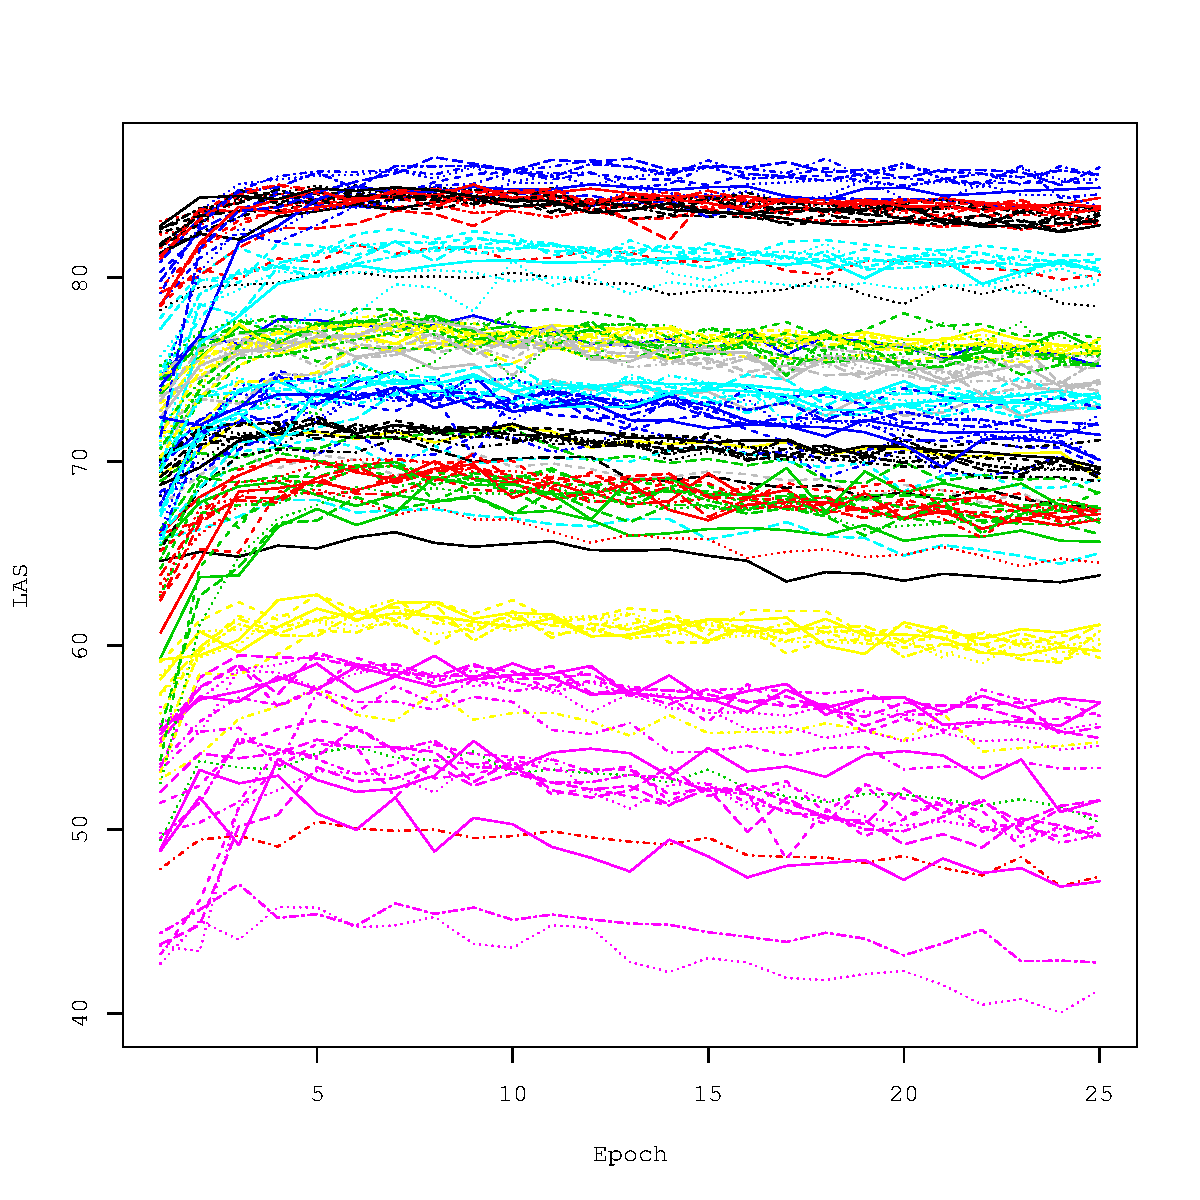
\includegraphics[width=\textwidth,page=1]{bachelor_thesis_plots.pdf}
  \caption[]{\label{fig:score:method}Training processes (excluding method~6). A color for each treebank.}
\end{figure}

For each treebank and each method,
we trained a model for 25 epochs on the train-set.
After each epoch, we took the model to parse the dev-set,
and calculated the LAS\@.%
\footnote{We also checked the unlabeled attachment scores (UAS) and came to the same judgments.
  The data are available in csv format:
  \url{https://github.com/ysmiraak/darc/tree/master/thesis/data}}

Method~6 was numerically unstable and failed to train for all but the Chinese treebank.
The reason why the Chinese treebanks was spared is clear from the \(\lceil\texttt{feats}\rceil\) column in Table~\ref{tab:ds:feats}.

Figure~\ref{fig:score:method} shows that for most processes,
no apparent over-fitting occurred, but mere slight fluctuations,
and that for most treebanks, the scores produced by different methods are extremely close.
For these reasons, we took the top three scores from each process,
instead of only the best ones.
This gives us more data points for analysis,
and also counters random luck whereby some processes happened to peak at the end of a training epoch
while others passed their peaks in the middle of an epoch.

\begin{figure}[htb!]
  \centering
  \includegraphics[width=\textwidth,page=2]{bachelor_thesis_plots.pdf}
  \caption[]{\label{fig:rank:method}Ranking of methods.}
\end{figure}

The scores are not comparable across treebanks,
and our goal was to investigate if some methods are consistently better than others.
Therefore instead of testing for each treebank whether one method is significantly better than another by some ad hoc definition of significance,
we simply compared the ranks.
The top three scores from each processes were ranked within each treebank,%
\footnote{Taking the top one score leads to the same judgments, only with the differences appearing to be more extreme.}
and the ranks were grouped by the methods.%
\footnote{The scores were rounded to two decimals. Equal scores were given equal ranks.}

In Figure~\ref{fig:rank:method},
the low position of the baseline method (0) shows that morphological features are helpful for all treebanks, including Chinese.
It is also evident that the binary methods (2--4), the normalized summed methods (8--9),
and the maxout method (10) are better than the others.
For the binary methods, normalization seems unnecessary,
while for the summed methods, \(L^{2}\)-normalization appears to have the best potential.

We picked the unnormalized binary method, the \(L^{2}\)-normalized summed method, and the maxout method for further investigations.
From this point forward,
the first two are simply referred to as the binary and the summed methods.

\section{Further investigations}
\label{sec:res2}

\begin{figure}[htb!]
  \centering
  \includegraphics[width=\textwidth,page=3]{bachelor_thesis_plots.pdf}
  \caption[]{\label{fig:rank:trial}\ttfamily\scriptsize
    \begin{tabular}{lc@{\enskip}c@{\enskip}c@{\enskip}c@{\enskip}c@{\enskip}c@{\enskip}c@{\enskip}c@{\enskip}c@{\enskip}c@{\enskip}c@{\enskip}c@{\enskip}c@{\enskip}c@{\enskip}c@{\enskip}c@{\enskip}c@{\enskip}c@{\enskip}c}
      trial &1 &2 &3 &4 &5 &6 &7 &8 &9 &10 &11 &12 &13 &14 &15 &16 &17 &18 &19\\
      \midrule
      binary &\(\bullet\) &&&\(\bullet\) &&&\(\bullet\) &&&\(\bullet\) &&&\(\bullet\) &&&\(\bullet\) &&&\\
      summed &&\(\bullet\) &&&\(\bullet\) &&&\(\bullet\) &&&\(\bullet\) &&&\(\bullet\) &&&\(\bullet\) &&\\
      maxout &&&\(\bullet\) &&&\(\bullet\) &&&\(\bullet\) &&&\(\bullet\) &&&\(\bullet\) &&&\(\bullet\) &\\
      +LEMMA &&&&\(\bullet\) &\(\bullet\) &\(\bullet\) &&&&\(\bullet\) &\(\bullet\) &\(\bullet\) &&&&\(\bullet\) &\(\bullet\) &\(\bullet\) &\(\bullet\)\\
      unit-norm &&&&&&&\(\bullet\) &\(\bullet\) &\(\bullet\) &\(\bullet\) &\(\bullet\) &\(\bullet\) &\(\bullet\) &\(\bullet\) &\(\bullet\) &\(\bullet\) &\(\bullet\) &\(\bullet\) &\(\bullet\)\\
      dropout &&&&&&&&&&&&&\(\bullet\) &\(\bullet\) &\(\bullet\) &\(\bullet\) &\(\bullet\) &\(\bullet\) &\(\bullet\)\\
    \end{tabular}}
\end{figure}

We continued the contest between the binary, the summed, and the maxout methods
while augmenting the model with lexical features and applying regularizations to the trainable embeddings.

For adding lexical features,
we tried two arrangements.

\begin{itemize}
  \ttfamily
\item FORM, \(64d\)-embedding
\item FORM \& LEMMA, \(32d\)-embedding each
\end{itemize}

This means that the dimension of the real vector space where we embed the lexical representations is fixed to 64.
The lexical space is either entirely dedicated to FORM,
or split between FORM and LEMMA\@.
This way the number of parameters in the first hidden layer stays constant.
Adding LEMMA on top of FORM actually decreases the total number of parameters,
because the LEMMA embedding matrix has fewer rows
(\texttt{\#form*} and \texttt{\#lemma*} in Table~\ref{tab:ds:stats}).

For applying regularizations to the trainable embeddings,
we tried three arrangements.

\begin{itemize}
  \ttfamily
\item Nothing
\item Unit-norm constraint
\item Unit-norm constraint, 25\% dropout
\end{itemize}

The unit-norm constraint normalizes the rows of the embedding matrix to unit vectors after each update.%
\footnote{The max-norm constraint may be a better option,
  which only enforces an upper bound on the norm.
  However, the optimal upper bound is a dataset-specific hyperparameter,
  which we wish to avoid.}

In total, we conducted 19 trials.
The ranking of the results are plotted in Figure~\ref{fig:rank:trial}.
The unit-norm constraint makes embedding training more effective (7--12 vs 1--6).
Dropout further helps (13--18 vs 7--12).
Without regularizations, adding LEMMA seems to have made no difference (4--6 vs 1--3);
It is however clearly superior, when regularizations are added (10--12 vs 7--9, 16--18 vs 13--15).
Trial 19 is the control group for 16--18,
without using inputs from FEATS\@.
It is evident that morphological features are helpful even with the presence of lexical features.

\begin{table}[htb!]
  \centering
  {\small
    \begin{tabular}{lc@{\enskip}c@{\enskip}cc@{\enskip}c@{\enskip}cc@{\enskip}c@{\enskip}c}
      \toprule
      &\multicolumn{3}{c}{\texttt{epoch}} &\multicolumn{3}{c}{\texttt{dev LAS}} &\multicolumn{3}{c}{\texttt{test LAS}}\\
      \texttt{treebank} &\texttt{b} &\texttt{s} &\texttt{m} &\texttt{b} &\texttt{s} &\texttt{m} &\texttt{b} &\texttt{s} &\texttt{m}\\
      \midrule
      \texttt{Ancient\_Greek} &18 &17 &18 &66.54 &\textbf{67.76} &\textsl{67.45} &66.25 &\textbf{67.23} &\textsl{67.10}\\
      \texttt{Arabic        } &10 &24 &17 &79.36 &\textsl{79.52} &\textbf{79.70} &78.05 &\textbf{79.23} &\textsl{79.17}\\
      \texttt{Basque        } &20 &19 &24 &76.61 &\textsl{77.35} &\textbf{77.44} &76.47 &\textsl{77.96} &\textbf{78.43}\\
      \texttt{Bulgarian     } &24 &16 &24 &88.20 &\textsl{88.91} &\textbf{89.17} &88.53 &\textsl{88.64} &\textbf{89.00}\\
      \texttt{Chinese       } &23 &24 &23 &\textsl{77.74} &77.43 &\textbf{77.79} &78.95 &\textsl{79.70} &\textbf{79.94}\\
      \texttt{Croatian      } &14 &24 &13 &81.94 &\textsl{82.25} &\textbf{82.41} &82.36 &\textsl{82.56} &\textbf{82.61}\\
      \texttt{Dutch         } &22 &20 &19 &82.78 &\textbf{83.34} &\textsl{83.14} &78.85 &\textsl{79.20} &\textbf{79.81}\\
      \texttt{Finnish-FTB   } &19 &24 &18 &\textbf{87.89} &87.53 &\textsl{87.63} &\textsl{86.95} &86.79 &\textbf{87.08}\\
      \texttt{Hebrew        } &23 &19 &14 &83.50 &\textsl{83.70} &\textbf{83.72} &\textsl{82.18} &\textbf{82.53} &81.81\\
      \texttt{Italian       } &20 &23 &19 &\textbf{88.94} &88.72 &\textsl{88.86} &\textsl{88.89} &\textbf{89.19} &88.76\\
      \texttt{Latin-PROIEL  } &16 &17 &23 &76.32 &\textbf{76.64} &\textsl{76.60} &74.90 &\textsl{74.97} &\textbf{76.68}\\
      \texttt{Persian       } &19 &19 &15 &\textsl{83.30} &83.21 &\textbf{83.54} &82.51 &\textbf{83.29} &\textsl{82.97}\\
      \texttt{Polish        } &13 &23 &23 &89.50 &\textsl{89.94} &\textbf{90.11} &88.98 &\textsl{90.05} &\textbf{90.41}\\
      \texttt{Swedish       } &14 &21 &15 &\textbf{81.62} &81.51 &\textbf{81.62} &\textbf{84.10} &83.96 &\textsl{84.08}\\
      \texttt{Turkish       } &~8 &20 &18 &62.23 &\textbf{62.99} &\textsl{62.95} &\textbf{62.96} &\textsl{62.92} &61.90\\
      \bottomrule
    \end{tabular}}
  \caption[]{\label{tab:best}Best dev models.\\
    \texttt{b}: binary, \texttt{s}: summed, \texttt{m}: maxout.}
\end{table}

We took the best three models (16--18) for each treebank,
picked the parameters from the epoch which yielded the best LAS on the dev-set,
and parsed the test-set.
The results listed in Table~\ref{tab:best} shows that in general
the maxout method outperforms the summed method which in turn outperforms the binary method.
In fact, the dimension of the entry embedding in the maxout and the summed methods can be tuned for a better performance.

\section{Conclusion}
\label{sec:conc}

We have shown that morphological information is valuable in transition-based dependency parsing,
and that a most effective and efficient way to encode morphological annotations is training an embedding from morphological entries to real vector space as part of the model,
and construct the vector representation for an AVS from its entries,
through scalar composition such as the max operation.

We participated in the CoNLL 2017 Shared Task with our parser, darc \parencite{yu2017parse},
and achieved results comparable to UDPipe 1.0 and 2.0 systems \parencite{udpipe},%
\footnote{\url{https://ufal.mff.cuni.cz/udpipe}}
despite the many limitations of our system in contrast.
We did lose to UDPipe 2.0,
however at the time, we applied the binary method without the knowledge that the maxout method would be better.
Table~\ref{tab:udpipe} compares the parsing scores of the two systems given the gold-standard segmentation and tagging information.

\begin{table}
  \centering
  {\small
    \begin{tabular}{lcccc}
      \toprule
      &\multicolumn{2}{c}{\texttt{UAS}} &\multicolumn{2}{c}{\texttt{LAS}}\\
      \texttt{treebank} &\texttt{UDPipe 2.0} &\texttt{darc maxout} &\texttt{UDPipe 2.0} &\texttt{darc maxout}\\
      \midrule
      \texttt{Ancient\_Greek} &69.2 &\textbf{71.6} &64.4 &\textbf{67.1}\\
      \texttt{Arabic        } &82.9 &\textbf{83.8} &77.9 &\textbf{79.2}\\
      \texttt{Basque        } &\textbf{82.3} &82.1 &78.4 &78.4\\
      \texttt{Bulgarian     } &\textbf{92.6} &92.1 &\textbf{89.1} &89.0\\
      \texttt{Chinese       } &\textbf{84.1} &82.8 &\textbf{81.4} &79.9\\
      \texttt{Croatian      } &\textbf{87.1} &86.6 &\textbf{83.2} &82.6\\
      \texttt{Dutch         } &82.9 &\textbf{83.7} &79.4 &\textbf{79.8}\\
      \texttt{Finnish-FTB   } &88.8 &\textbf{89.2} &86.5 &\textbf{87.1}\\
      \texttt{Hebrew        } &\textbf{87.8} &85.6 &\textbf{84.3} &81.8\\
      \texttt{Italian       } &\textbf{91.3} &90.4 &\textbf{89.7} &88.8\\
      \texttt{Latin-PROIEL  } &79.0 &\textbf{80.2} &75.0 &\textbf{76.7}\\
      \texttt{Persian       } &\textbf{87.7} &86.0 &\textbf{84.9} &83.0\\
      \texttt{Polish        } &92.9 &\textbf{93.4} &89.5 &\textbf{90.4}\\
      \texttt{Swedish       } &\textbf{88.0} &87.1 &\textbf{85.0} &84.1\\
      \texttt{Turkish       } &66.8 &\textbf{67.3} &61.1 &\textbf{61.9}\\
      \midrule
      \texttt{average       } &\textbf{84.2} &84.1 &80.7 &80.7\\
      \bottomrule
    \end{tabular}}
  \caption[]{\label{tab:udpipe}Darc vs UDPipe.}
\end{table}

Better parsing algorithms and architectures have been proposed,
and our method for encoding morphological annotations is applicable to any neural network models.
However, good morphological annotations may not always be available.
\textcite{bojanowski2016enriching} proposed a method for constructing morphological word representations
by learning representations for character n-grams and composing words as the sum.
Their method extracts morphological information directly from the orthography,
a natural source of linguistic annotations,
and our method utilizes an external source, namely the morphological tags.
Both methods compose the vector representation for a complex structure
from the vector representations of its components by an componentwise operation.
This approach is generally worth considering in machine learning where some input comes with polymorphic information,
such as instances with soft clusters or types with type classes.

\printbibliography[]

\end{document}
% LocalWords:  Çağrı Çöltekin UD nonp fus agg FTB DEPREL upos drel UPOSTAG Darc
% LocalWords:  xcomp det nsubj obl punct darc VerbForm XPOSTAG DEPS Pos CCONJ rl
% LocalWords:  PronType Plur relcl hs psor MaltParser UDPipe ud testdata nivre
% LocalWords:  udst chen chollet whitepaper kingma srivastava mikolov VerbType
% LocalWords:  udparsing goodfellow alberti bojanowski antiplagiatserklaerung
% LocalWords:  DET PUNCT
